\chapter{その他の機能}

\section{複数のファイルに分割してある文章について}

TeXstudioでは、複数ファイルに分割された文書を扱うことができる。

TeXファイルを文書に含めるためには、
「LaTeX」メニューの「\verb+\include{file}+」または
「\verb+\input{file}+」コマンドを使用すれば良い。
そのファイルは「構造ビュー」に表示されることになる。
そのファイル名をクリックすることで、TeXstudioでそのファイルを開くことができる。

TeXstudioは今や読み込んだ文書の親/子関係を理解する(1レベルのみ!)。
従って「マスター文書モード」でのように、
子の文書について作業している間コンパイルを開始すると親文書のみがコンパイルされる。
また、対応する全ての文書内のラベルとユーザーコマンドが認識される。

更に、「オプション」メニューで「マスターファイル」を定義することもできる。
「子」文書に対して作業している時でさえ、
「ツール」メニューのコマンド全てはマスターファイルに対してのみ
適用される(「マスター」ファイルを閉じることすら可能である)。

マスターファイルが設定されている場合、
開いてある文書で定義されているラベルとユーザーコマンドは
開いてある文書全てで補完候補として利用できる。
従って、別のサブ文書で定義されているラベルへの参照を
その文書をTeXstudioで開いている限り簡単に挿入できる。

注:「オプション」メニューで「マスター」モードを解除できる。

\section{構文チェック}

LaTeX構文チェッカーは、
コマンドが正しいかどうか決めるため考えられる補完コマンドのリストを採用している。
どの文脈でコマンドが有効であるか、
例えばコマンドが数式モードでのみまたは表モードでのみ有効なのかどうかを決めるため、
補完リストは部分的に追加情報を含んでいる。

更に表の正確さはより詳細に確認される。
列の数が続く行で解析・確認される。
もしある行で列の数が多かったり少なかったりすると、警告印が表示される。

\section{参考文献}

``bib''ファイルに対して、
「文献」メニューで文書の標準型に対応する項目を直接挿入できる。

注:「文献」メニューの「削除」コマンドでオプション項目が自動的に削除される。

\begin{figure}[H]
  \centering
  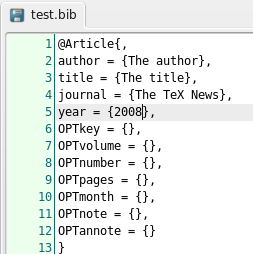
\includegraphics{doc16.png}
  \caption{参考文献}
\end{figure}

\section{SVNサポート}\label{sec:svnsupport}

%第1.8節
第\ref{sec:config_svn}節(\nameref{sec:config_svn})ですでに述べた
サポートされているsvn機能とは別に、
TeXstudioはさらに2つのコマンドをサポートしている。

「ファイル/SVN/チェックイン」で、
svn履歴に保存されるチェックインメッセージを求める入力ダイアログとともに
明示的に保存、チェックインが行われる。

「ファイル/SVN/古いリビジョンを表示」で、
全ての利用可能なリビジョンを表示するダイアログが表示される。
古いリビジョンを選択することで、その古いリビジョンへ現在の文書が即座に変更される。
また、古い部分をコピーして最新のバージョンへ戻ることで、
その部分を文書の最新バージョンにすることができる。
もしその文書を直接編集し始めると、
ダイアログは閉じて現在のテキストが未保存だが新しい最新バージョンとなる。

\section{私的マクロ}

TeXstudioでは自分のマクロを挿入できる
(ショートカット:Shift+F1\ldots{}Shift+F10)。
これらのマクロは「マクロ - マクロを編集」メニューで定義できる。
マクロはTXSに直接配置される単純なテキストからなる。
また、それはbegin/endで自動的に展開される「環境」でも、
java scriptでも良い。
必要な機能はチェックボックスで選択することができる。

「略語」はLaTeX補完に対する擬似コマンドである。
擬似コマンドが補完されると代わりにそのマクロが挿入される。
擬似コマンドはバックスラッシュ(``\textbackslash{}'')で始まる必要があることに注意すること。

「トリガー」はマクロを含むものを自動実行する正規表現である:
最後に入力された文字がこの表現に一致すると、
それは削除されてマクロが挿入/実行される(詳細は
%\hyperref[sectionTriggers]{下}
\nameref{sec:triggers}を見ること)。

\begin{figure}[H]
  \centering
  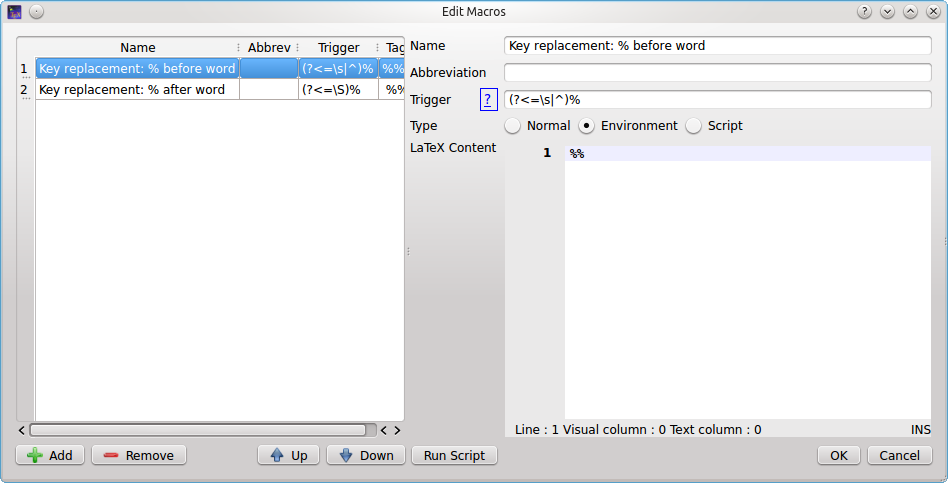
\includegraphics[width=.8\linewidth]{doc17.png}
  \caption{マクロの編集}
\end{figure}

\subsection{テキストマクロ}

通常のテキストとは別に、いくつかの特別なコードが認識されて挿入時に置換される。

もしどこかに\verb+%|+を書いた場合、
カーソルは挿入されたテキストのその場所に配置される
(2番めの\verb+%|+はそれらの間全ての選択になる)。

\verb+%<something%>+を書くと、
Ctrl+Left/Rightで選択できる説明的テキストとしてしるし付けされる。

オプション\texttt{\%(\emph{filefilter}\%)}は
ファイルダイアログで尋ねられるファイル名で置換される。
ファイルフィルター\emph{filefilter}は標準的なQtファイルフィルター形式である。

例:``Images (*.png *.xpm *.jpg);;Text files (*.txt);;XML files (*.xml)''。
\href{http://qt-project.org/doc/qt-4.8/qfiledialog.html\#getOpenFileName}{Qt-Doc}も参照すること。

\subsection{環境マクロ}

テキストは環境名として用いられる。
従って``\verb+%environment+''は次のように挿入される:

\begin{lstlisting}[frame=single]
\begin{environment}

\end{environment}
\end{lstlisting}

注:TeXstudioでは、挿入時に配置されないものの環境名が``\%''で始まる必要がある。

\subsection{Javascriptマクロ}

コード片を用いる代わりに、javascriptを使用することもできる。
そのためには最初の行に``\verb+%SCRIPT+''を置けばよい。
続くコードはjavascriptとして解釈される。
言語は\href{http://www.ecmascript.org/index.php}{ECMAScript}に基づく。
文書にアクセスするために次のオブジェクトが導入されている:

\begin{itemize}
\item
  ``editor''で検索/保存/読み込みといった最上位の操作を現在の文書で行うことができる。
\item
  ``cursor''で移動、テキストの挿入や削除といったカーソル操作にアクセスすることができる。
\item
  ``fileChooser''で非常に単純なファイル選択ダイアログにアクセスすることができる。
\item
  ``app''でクリップボードやメニューといったアプリケーションの幅広いものへアクセスすることができる。
\end{itemize}

次の表は考えられるコマンドの概要である。

\begin{table}[H]
  \centering
  \caption{グローバルスコープのコマンド一覧}
  \begin{tabularx}{\linewidth}{XX}
    \hline
    \multicolumn{2}{c}{\textbf{グローバルスコープ}}\\
    \textbf{コマンド} & \textbf{説明}\\
    \hline
    \texttt{alert(str)}, \texttt{information(str)}, \texttt{warning(str)}
    または\texttt{critical(str)}
      & 文字列\texttt{str}をあるアイコンとともにメッセージボックスに表示\\
    \texttt{confirm(str)}または\texttt{confirmWarning(str)}
      & 文字列\texttt{str}をはい/いいえ(yes/no)の質問として
      メッセージボックスに表示\\
    \texttt{debug(str)} & 文字列\texttt{str}を標準出力stdoutに表示\\
    \texttt{writeFile(name, value)}
      & ファイル\texttt{name}に値\texttt{value}を書き込む(書き込み権限を要求)\\
    \texttt{readFile(name)}
      & ファイル\texttt{name}全体を読み込む(読み込み権限を要求)\\
    \texttt{system(cmd)}
      & コマンド\texttt{cmd}を呼び出し、
      次のメソッドをもつProcessXオブジェクトを返す:
      \begin{itemize}
      \item
        \texttt{waitForFinished}: プロセスが終了するまで待つ
      \item
        \texttt{readAllStandardOutputStr}: 標準出力stdoutを返す
      \item
        \texttt{readAllStandardErrorStr}: 標準エラー出力stderrを返す
      \item
        \texttt{exitCode}: 終了コード
      \item
        \texttt{exitStatus}: Qt終了ステータス
      \item
        \texttt{terminate}または\texttt{kill}: プロセスを停止する
      \end{itemize}\\
    \texttt{setGlobal(name, value)} & 一時的なグローバル変数を設定する\\
    \texttt{getGlobal(name)} & グローバル変数を読み込む\\
    \texttt{hasGlobal(name)} & グローバル変数の存在を確認する\\
    \texttt{setPersistent(name, value)}
      & グローバル設定変数を設定する(iniファイルの値を変更することができる。
      書き込み権限を要求)\\
    \texttt{getPersistent(name)}
      & グローバル設定変数を読み込む(iniファイルの値全てを読み込むことができる。
      読み込み権限を要求)\\
    \texttt{hasPersistent(name)}
      & グローバル設定変数が存在するかを確認する(読み込み権限を要求)\\
    \texttt{hasReadPrivileges()} & スクリプトに読み込み権限があるかを確認する\\
    \texttt{hasWritePrivileges()} & スクリプトに書き込み権限があるかを確認する\\
    \texttt{registerAsBackgroundScript({[}id{]})}
      & スクリプトがバックグラウンドで実行できるようにする
      (スクリプトがイベント/シグナルを扱う場合には必要)\\
    \texttt{triggerMatches}
      & スクリプトがエディタ\nameref{sec:triggers}で呼び出された場合、
      通常のトリガー表現に一致する\\
    \texttt{triggerId}
      & スクリプトがイベント\nameref{sec:triggers}で呼び出された場合、
      トリガーのidの数字を表す\\
    \texttt{include(script)}
      & 別のスクリプトを読み込む。scriptはファイル名やマクロ名である。\\
    \texttt{pdfs} & 全ての開いている内部pdfビューワーのリストである\\
    \hline
  \end{tabularx}
\end{table}

\LTXtable{\linewidth}{editobjtab}

\begin{table}[H]
  \centering
  \caption{文書オブジェクトの一覧}
  \begin{tabularx}{\linewidth}{XX}
    \hline
    \multicolumn{2}{c}{\textbf{文書オブジェクト}}\\
    \textbf{コマンド} & \textbf{説明}\\
    \hline
    \texttt{editor.document().lineCount()} & 行の数を返す\\
    \texttt{editor.document().visualLineCount()}
      & 見かけの行の数を返す(ワードラップした行を数える)\\
    \texttt{editor.document().cursor(line, {[}column = 0{]}, {[}lineTo = -1{]}, {[}columnTo = length of lineTo{]})}
      & カーソルオブジェクトを返す。
      もし\texttt{lineTo}が与えられた場合、
      カーソルは\texttt{line:column}から\texttt{lineTo:columnTo}までの選択部を持つ。\\
    \texttt{editor.document().text({[}removeTrailing = false{]}, {[}preserveIndent = true{]})}
      & 文書のテキスト全体を返す\\
    \texttt{editor.document().textLines()} & テキスト行全ての配列を返す\\
    \texttt{editor.document().lineEndingString()}
      & 行の末端(\verb+\n+または{\verb+\n\r+})を含む文字列を返す\\
    \texttt{editor.document().canUndo()} & 元に戻す(undo)が可能なら真(true)を返す\\
    \texttt{editor.document().canRedo()} & やり直す(redo)が可能なら真(true)を返す\\
    \texttt{editor.document().expand(lineNr)} & 行を展開する\\
    \texttt{editor.document().collapse(lineNr)} & 行を折りたたむ\\
    \texttt{editor.document().expandParents(lineNr)}
      & 行の全ての親をその行が見えるまで展開する\\
    \texttt{editor.document().foldBlockAt(bool unFold, lineNr);}
      & \texttt{lineNr}の前の最初のブロックを折りたたむまたは展開する\\
    \texttt{editor.document().getMasterDocument();}
      & この文章を直接含む開いてある文書を返す\\
    \texttt{editor.document().getTopMasterDocument();}
      & この文章を間接的に含み、自身は他の文書で含まれていない、
      開いてある文書を返す\\
    \texttt{editor.document().getMagicComment(name);}
      & 存在する場合マジックコメントの内容を返す\\
    \texttt{editor.document().updateMagicComment(name, value, {[}create = false{]});}
      & マジックコメントを変更する\\
    \texttt{editor.document().labelItems/refItems/bibItems}
      & 全てのラベル/参照または含まれる参考文献ファイルのidを返す\\
    \hline
  \end{tabularx}
\end{table}

\begin{table}[H]
  \centering
  \caption{文書管理オブジェクトの一覧}
  \begin{tabularx}{\linewidth}{lX}
    \hline
    \multicolumn{2}{c}{\textbf{文書管理オブジェクト}}\\
    \textbf{コマンド} & \textbf{説明}\\
    \hline
    \texttt{documentManager.currentDocument}
      & 現在の文書(スクリプトがバックグラウンドモードで起動していない限り、
      通常は\texttt{editor.document()}と同じである)\\
    \texttt{documents.masterDocument} & マスターファイル\\
    \texttt{{[}documentManager.{]}documents} & 開いている文書全ての配列\\
    \texttt{documentManager.findDocument(fileName)}
      & あるファイル名\texttt{fileName}を持つ開いてある文書を返す\\
    \texttt{documentManager.singleMode()}
      & 明示的なマスターファイルがない場合真(true)を返す\\
    \texttt{documentManager.getMasterDocumentForDoc(document)}
      & 与えられた文書(\texttt{document})を
      (おそらく間接的に)含んでいる開いてある文書を返す\\
    \texttt{documentManager.findFileFromBibId(id)}
      & 与えられた\texttt{id}の項目を含むbibファイルのファイル名を返す\\
    \hline
  \end{tabularx}
\end{table}

\LTXtable{\linewidth}{cursorobjtab}

\begin{table}[H]
  \centering
  \caption{アプリケーションオブジェクトの一覧}
  \begin{tabularx}{\linewidth}{lX}
    \hline
    \multicolumn{2}{c}{\textbf{アプリケーションオブジェクト}}\\
    \textbf{コマンド} & \textbf{説明}\\
    \hline
    \texttt{app.getVersion()} & 現在のバージョン(0xMMmm00)\\
    \texttt{app.clipboard} & クリップボードへの読み書きのための属性\\
    \texttt{app.getCurrentFileName()} & 現在編集しているファイルの名前\\
    \texttt{app.getAbsoluteFilePath(rel, ext = "")}
      & 相対的なファイル名を絶対的なものに変換する\\
    \texttt{app.load(file)} & ファイル\texttt{file}を読み込む\\
    \texttt{app.fileOpen/Save/Close/\ldots{}/editUndo/\ldots{}/QuickBuild/\ldots{}}
      & メニューコマンド全て(つまりtexmaker.hファイルのスロット全て)。
      設定ダイアログの「メニュー」ページの現在存在する
      スロット全てのリストを見ることができる。\\
    \texttt{app.newManagedMenu({[}parent menu,{]} id, caption)}
      & 新規メニューを作成してそれを返す\\
    \texttt{app.getManagedMenu(id)}
      & ある\texttt{id}を
      持つ\href{http://developer.qt.nokia.com/doc/qt-4.8/QMenu.html}{QMenu}を返す\\
    \texttt{app.newManagedAction(menu, id, caption)}
      & 新規アクションを作成してそれを返す
      \begin{itemize}
      \item
        \texttt{menu}: 親メニュー
      \item
        \texttt{id}:
        新規アクションのID(最後の唯一のIDは\emph{メニューid/アクションid}となる)
      \item
        \texttt{caption}: 表示されるテキスト
      \end{itemize}

      \texttt{action.triggered.connect(function()\{ \ldots{}\});}を用いて、
      関数を返りアクションへつなげることができる
      (詳細は\href{http://developer.qt.nokia.com/doc/qt-4.8/scripting.html\#signal-to-function-connections}{qt signal/slot}文書を見ること)。\\
    \texttt{app.getManagedAction({[}id{]})}
      & ある\texttt{id}を持つ
      \href{http://developer.qt.nokia.com/doc/qt-4.8/QAction.html}{QAction}を
      返す(全てのidは通常
      一つのメニューでmain/menu1/menu2/\ldots{}/menuN/actionという形を持つ。
      例:``main/edit/undo''。texmaker.cppを見ること。)\\
    \texttt{app.createUI(file, {[}parent{]})}
      & あるuiファイルを読み込み、それからQWidget*を作成する\\
    \texttt{app.createUIFromString(string, {[}parent{]})}
      & 文字列\texttt{string}で記述されたQWidget*を作成する\\
    \texttt{app.slowOperationStarted()/slowOperationEnded()}
      & 遅い操作の開始/終了に関して一時的に無限ループ検出を
      無効化するようTXSに通知する\\
    \hline
  \end{tabularx}
\end{table}

\begin{table}[H]
  \centering
  \caption{UniversalInputDialogクラスの一覧}
  \begin{tabularx}{\linewidth}{XX}
    \hline
    \multicolumn{2}{c}{\textbf{UniversalInputDialogクラス}}\\
    \textbf{コマンド} & \textbf{説明}\\
    \hline
    \texttt{new UniversalInputDialog()} & 新しいダイアログを作成する\\
    \texttt{dialog.add(defaultValue, {[}description, {[}id{]}{]})}
      & 与えられた規定値\texttt{defaultValue}と
      省略可能な説明\texttt{description}と\texttt{id}を持つ新しい変数を
      ダイアログに追加する。
      そして対応するQtコンポーネントを返す。\newline
      文字列既定値はQLineEditに、数字はQSpinBoxに、配列はQComboBoxになる。\\
    \texttt{dialog.get(nr/id)}
      & \texttt{nr}番目に追加された変数または
      ある\texttt{id}を持つ変数の現在値を返す\\
    \texttt{dialog.getAll()}
      & 全ての変数の値を組み合わされた数字/連想配列として返す。
      i番目の変数を得るために\texttt{returnvalue{[}i{]}}を、
      あるidを持つ変数を得るために\texttt{returnvalue.id}を用いることができる。\\
    \texttt{dialog.exec()}
      & ダイアログを表示する。
      ユーザーが取り消した場合nullを返し、
      ユーザーが承諾した場合\texttt{getAll()}の値を返す。\\
    \texttt{dialog.show()} & ダイアログを非同期的に表示する\\
    \texttt{UniversalInputDialog({[}{[}defaultValue\_0, description\_0, id\_0{]}, {[}defaultValue\_1, description\_1, id\_1{]}, \ldots{}{]})}
      & 短い形:新規ダイアログを作成して、配列の全ての変数を追加し、
      \texttt{exec}をその上で呼び出す\\
    \hline
  \end{tabularx}
\end{table}

\begin{table}[H]
  \centering
  \caption{FileChooserオブジェクトの一覧}
  \begin{tabularx}{\linewidth}{XX}
    \hline
    \multicolumn{2}{c}{\textbf{FileChooserオブジェクト}}\\
    \textbf{コマンド} & \textbf{説明}\\
    \hline
    \texttt{fileChooser.exec()} & ダイアログを表示して、再度閉じられるまで待機する\\
    \texttt{fileChooser.setDir(dir)}
      & ダイアログ内のディレクトリを\texttt{\emph{dir}}に設定する\\
    \texttt{fileChooser.setFilter(filter)}
      & QT-formatを用いてファイルフィルターを\texttt{\emph{filter}}に設定する。
      上を参照すること。\\
    \texttt{fileChooser.fileName()} & (execの後)選択したファイル名を返す\\
    \hline
  \end{tabularx}
\end{table}

いくつかの例:

\begin{itemize}
\item
  現在のファイル名をクリップボードにコピーする:
\begin{lstlisting}[frame=single,language=JavaScript,numbers=left]
%SCRIPT
app.clipboard = editor.fileName();
\end{lstlisting}
\item
  エディタテキストの実行:
\begin{lstlisting}[frame=single,language=JavaScript,numbers=left]
%SCRIPT
eval(editor.text());
\end{lstlisting}
\item
  オブジェクトの全ての属性を表示する:
\begin{lstlisting}[frame=single,language=JavaScript,breaklines=true,numbers=left]
%SCRIPT
obj = editor;                                                    //表示するオブジェクト(例:現在のエディタ)

app.fileNew();                                                   //新しい文書を作成
newEditor = documentManager.currentDocument.editorView.editor;   //新しく作成された文書にアクセス
for (var prop in obj)
  newEditor.write(prop+"\n");                                    //属性を出力
\end{lstlisting}
\item
  編集メニューにアクションを追加:
\begin{lstlisting}[frame=single,language=JavaScript,breaklines=true,numbers=left]
%SCRIPT
var menu = app.getManagedMenu("main/edit");                   //編集メニューを入手
var act = app.newManagedAction(menu, "script", "scripttest"); //アクションを追加
act.triggered.connect(function(){alert("called");});          //簡単なハンドラを登録
registerAsBackgroundScript("test");                           //ハンドラを有効化し続ける
\end{lstlisting}
\item
  非同期ダイアログ:
\begin{lstlisting}[frame=single,language=JavaScript,breaklines=true,numbers=left]
%SCRIPT
var ui = createUI(" ... path to your ui file ...");  //ダイアログを読み込む
ui.accepted.connect(function(){alert("x");})         //ダイアログを閉じることに反応
registerAsBackgroundScript("abc");                   //関数の有効化を維持
ui.show();                                           //ダイアログの表示
\end{lstlisting}

  ダイアログはQt Designerで作られるuiファイルに記述されている。
\item
  計算機:
\begin{lstlisting}[frame=single,language=JavaScript,breaklines=true,numbers=left]
%SCRIPT
currentLine=editor.text(cursor.lineNumber());
from=currentLine.lastIndexOf("%")+1;
to=currentLine.lastIndexOf("=");
if (from>=0 && to > from) {
  toEvaluate = currentLine.substring(from, to);
  with (Math) { value = eval(toEvaluate);}
  cursor.eraseLine();
  cursor.insertText(currentLine.substring(0, from)+toEvaluate+"="+value);
  cursor.insertLine();
  cursor.movePosition(1,cursorEnums.Left );
}
\end{lstlisting}

  これは\%と=の間のもの全てを評価して、=の後ろに結果を書き込む。
  texファイルに\%5+3=を書くと計算機のように使用出来る。
\item
  (tikz)座標の組の移動:
\begin{lstlisting}[frame=single,language=JavaScript,breaklines=true,numbers=left]
%SCRIPT
var doit = function(){
  var mytext=cursor.selectedText();
  var regExNumberPre = " *[0-9]+([.][0-9]*)? *";
  var regExDigit = /[0-9]/;
  var regExSpace = / /g;
  var regExPairPre = " *(-?"+regExNumberPre+")";
  var regExPair = new RegExp("()[(]"+regExPairPre+","+regExPairPre+"[)]"); ;

  //最初の座標の組を読み込む
  var regExFirstPairPre = regExPairPre + " *([+-]"+regExNumberPre+")?";
  var regExFirstPair = new RegExp("()[(]"+regExFirstPairPre+","+regExFirstPairPre+"[)]");

  //オフセットを抽出(-x - yを許可するため、最初の数字から正規表現検索を開始)
  var matches = regExFirstPair.exec(mytext);
  if (matches == null) throw "missing";
  //一致物を投げる
  var offsetXPre = matches[4];
  var offsetYPre = matches[8];
  if (offsetXPre == "" && offsetYPre == "") throw "abc";
  var offsetX = offsetXPre == ""?0.0:offsetXPre.replace(regExSpace, "")*1.0;
  var offsetY = offsetYPre == ""?0.0:offsetYPre.replace(regExSpace, "")*1.0;

  //最初の組を移動
  var matchpos = mytext.search(regExFirstPair);
  editor.write(mytext.slice(0,matchpos));
  editor.write("("+(matches[2].replace(regExSpace, "")*1.0+offsetX));
  editor.write(", "+(matches[6].replace(regExSpace, "")*1.0+offsetY)+")");

  //他の組を移動
  var remaining = mytext.slice(matchpos+matches[0].length);
  while (remaining != ""){
    matches = regExPair.exec(remaining);
    if (matches == null) break;
    matchpos = remaining.search(regExPair);
    editor.write(remaining.slice(0,matchpos));
    remaining = remaining.slice(matchpos+matches[0].length);
    editor.write("(" + ((matches[2].replace(regExSpace, "")*1.0)+offsetX) + ", "+ ((matches[4].replace(regExSpace, "")*1.0)+offsetY) + ")");
  }
editor.write(remaining);
}
doit();
\end{lstlisting}

  これは、全ての選択した座標の組に最初の組のオフセットを加えて
  与えられた方向に全ての組を移動させる。
  例:($1 + 1$, $2 - 1.5$) (3, 4)がある場合、(2, 0.5) (4, 2.5)に変更される。
\end{itemize}

\subsection{トリガー}\label{sec:triggers}

トリガーの最も単純な形式では、トリガーは単なるテキストであり、マクロで置換される。
例:trigger=``eg'' macro=``example given''の場合、
``the leg''の``eg''は``g''を入力すると``example given''で置換される。

トリガーが正規表現であると、手の込んだトリガーを作成することができる。
TXSは後方参照検索を使用している:
``\verb+(?<=\s)%+''は、前の文字が空白なら``\%''を置換するのに使用される。
正規表現についてのさらなるヘルプはインターネット上で見ることができる。

また特定の言語(``latex''のような、例:\verb+(?language:latex)+)の文書でのみ
マクロを起動するために、擬似表現\verb+(?language:...)+を追加することもできる。

別のこうした前に追加可能なオプションは\verb+(?highlighted-as:..)+である。
これはマクロを特定の強調表示された環境に制限する
(例:\verb+(?highlighted-as:numbers,math-delimiter,math-keyword)+で、
マクロは数式モード中でのみ有効化される)。
可能な値は構文強調表示設定ページのリスト(英語)に一致する。

さらに、対応するイベントが生じた時にスクリプトを実行するために
次の特別なトリガー表現(括弧なし)を使うことができる:

\begin{table}[H]
  \centering
  \caption{特別なトリガー表現の一覧}
  \begin{tabularx}{\linewidth}{lX}
    \hline
    \texttt{?txs-start} & TeXstudio開始時\\
    \texttt{?new-file} & 新規ファイル作成時\\
    \texttt{?new-from-template} & テンプレートからの新規ファイル作成時\\
    \texttt{?load-file} & ファイル読み込み時\\
    \texttt{?load-this-file}
      & マクロを含むファイルの読み込み時(スクリプトが
      \hyperref[sec:magiccomment]{マジックコメント}として定義されている場合に
      のみ意味をなす)\\
    \texttt{?save-file} & ファイル保存時\\
    \texttt{?close-file} & ファイルを閉じた時\\
    \texttt{?master-changed} & 文書がマスターファイルとして定義解除/定義された時\\
    \texttt{?after-typeset} & LaTeX類似コマンド終了時\\
    \texttt{?after-command-run}
      & コマンド実行終了時(例:latexを2回呼び出して
      ビューワーを開くコンパイルコマンドの場合、このイベントが生じるのは
      1回だが\texttt{after-typeset}では2回である。)\\
    \hline
  \end{tabularx}
\end{table}

これら特殊トリガーは``\textbar{}''記号で複数個組み合わせることができる。

\section{Pstricksのサポート}

主なpstricksコマンドは「構造ビュー」の「Pstricks」パネルで挿入できる。

\section{Metapostのサポート}

Metapostキーワードは「構造ビュー」の「Metapost」パネルで挿入できる。
また、「ツール/コマンド」メニューを通じて「mpost」などのコマンドを
起動させることができる。

\section{「HTMLへ変換」コマンド}

このコマンド(「ツール」メニューにある)は、
LaTeXソースファイルからhtmlページ各々につき一画像のhtmlページのセットを生成する。
プレゼンテーションスライドの各ページは、
LaTeXを実行して得られるpostscriptページの一つに対応する。

またこのコマンドでは、LaTeXで得られる目次に対応するページも生成される。
このページの各項目は対応するhtmlページへのリンクを含んでいる。

texファイルに\verb+\ttwplink{}{}+コマンドを用いることで、
生成されるhtmlページにリンクを作成することができる。

概要:

\verb+\ttwplink{http://www.mylink.com}{my text}+ (外部リンク)

\verb+\ttwplink{page3.html}{my text}+ (内部リンク)

\verb+\ttwplink{name_of_a_label}{my text}+ (内部リンク)

\textbf{警告:}hyperrefパッケージ(あるいは他のいくつかのパッケージ)とともに
このコマンドを使用することはできない。
このコマンドは「HTMLへ変換」ツールとともにしか使用できない。

\begin{figure}[H]
  \centering
  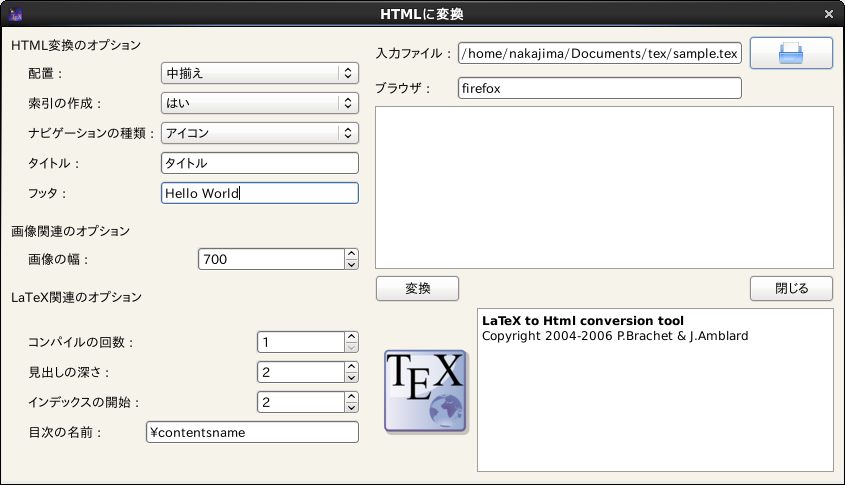
\includegraphics[width=.8\linewidth]{doc18.png}
  \caption{「HTMLへ変換」ダイアログ}
\end{figure}

\begin{figure}[H]
  \centering
  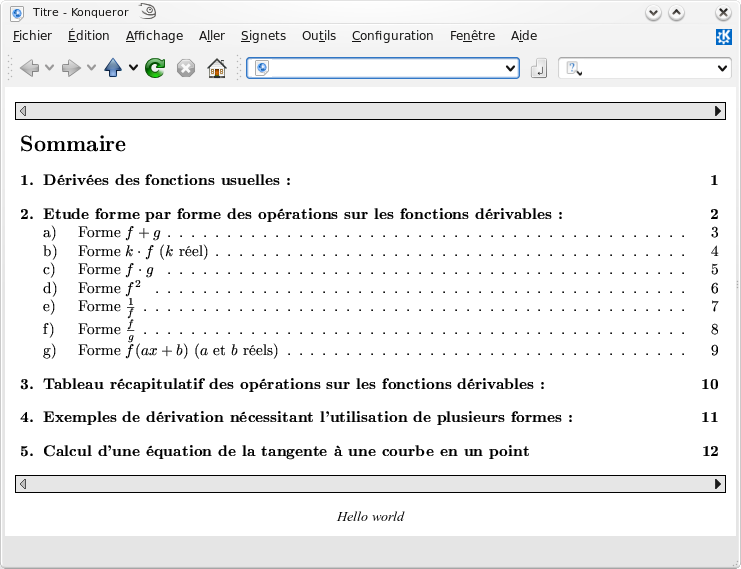
\includegraphics[width=.8\linewidth]{doc19.png}
  \caption{変換されたhtml}
\end{figure}

\section{TeXstudioでの「順方向/逆方向検索」}\label{sec:search}

\subsection{統合されたPDFビューワー}

TeXstudioでは順方向・逆方向検索を提供する統合されたPDFビューワーが提供されている。
pdflatexコマンド(または類似コマンド)でsynctexが有効化されていることを
確認すること(オプション``\texttt{-synctex=1}''を追加する必要がある)。
もし正しく設定されていない場合、
TeXstudioはコマンド自体を修正するかどうかを尋ねる。

順方向検索はPDFビューワーが開いた時にはいつも自動的に行われる。
TeXstudioはカーソルが現在位置している場所へ(PDF上で)移動する。
さらに、テキストエディタ上の単語をCTRL+左クリックすることでPDFへ移動したり、
コンテキストメニューを用いて「PDFへ移動」を選択して移動することもできる。

逆方向検索は、PDF上でCTRL+左マウスボタンクリックするか、
コンテキストメニュー(右マウスボタンクリック)で「ソースへ移動」を選択することで
有効になる。
さらに、PDFビューワーの設定で「カーソルに続いてスクロールする」を
有効化することができる。
これで、PDFビューワー上の位置をエディタ上のカーソル位置に同期させることができる。
同様に、「スクロールに続いてカーソルを移動する」を有効化することで
エディタ上の位置をPDFビューワー上の位置に同期させることができる。

\subsection{外部ビューワーに対する一般的な設定}

いくつかの(dvi)ビューワーでは、
(La)TeXソースファイル上のある行番号に対応するDVIファイル上での位置へ移動
(あるいは視覚的に強調表示)することができる。

この順方向検索を有効にするには、
ユーザーツール(「オプション/TeXstudioの設定」 -\textgreater{} 「ビルド」)の
コマンド行または設定ダイアログのビューワーコマンド行
(「オプション/TeXstudioの設定」 -\textgreater{} 「コマンド」)で、
対応するビューワーのコマンドを入力すれば良い。
ビューワーが起動するときに、\textbf{@}プレースホルダは現在の行番号で置換され、
\textbf{?c:ame}は現在のファイルの完全な絶対パスでのファイル名で置換される。\\


Windowsでは、次の形のコマンドを挿入することでDDEコマンドを実行できる:
\texttt{dde:///service/control/{[}commands\ldots{}{]}}
あるいは必要な場合次の形のコマンドでプログラムを起動することもできる
(TeXstudio 1.9.9から):
\texttt{dde:///programpath:service/control/{[}commands\ldots{}{]}}\\


下にいくつかの一般的なビューワーに対するコマンドのリストを載せている。
当然、コマンドを使用したい場合\emph{(your program path)}を
コンピュータ上のそのプログラムのパスで置換する必要がある。

\subsection{Sumatra}

SumatraをTeXstudioから起動して逆方向検索を設定:
\texttt{"\emph{(your sumatra path)}" -reuse-instance -inverse-search
 """"\emph{(your TeXstudio path)}""" """\%\%f""" -line \%\%l" "?am.pdf"}\\


起動しているSumatraである行へ移動(Windows限定):\\
\texttt{dde:///SUMATRA/control/{[}ForwardSearch("?am.pdf","?c:am.tex",@,0,0,1){]}}\\


起動していなければSumatraを実行して、ある行へ移動(Windows限定):
\texttt{dde:///\emph{(your sumatra path)}:SUMATRA/control/{[}ForwardSearch("?am.pdf","?c:am.tex",@,0,0,1){]}}\\


SumatraからTeXstudioを実行: \texttt{"\emph{(your TeXstudio path)}" "\%f" -line \%l}\\


\emph{(your Sumatra path)}の考えられる値は
\verb+C:/Program Files/SumatraPDF/SumatraPDF.exe+である。

\subsection{Foxit Reader}

Foxit ReaderをTeXstudioから起動:
 \texttt{"\emph{(your Reader path)"} "?am.pdf"}

\subsection{Acrobat Reader}

TeXstudioからAcrobat Readerを起動:
 \texttt{"\emph{(your Reader path)"} "?am.pdf"}\\


移動と閉じることはDDEコマンドを通じて行う。
Adobe製品のバージョン10から、DDEサービス名に製品とバージョン番号に対する文字列が含まれる。

\begin{table}[H]
  \centering
  \caption{製品とサービス名の対応}
  \begin{tabular}{ll}
    \hline
    \textbf{製品} & \textbf{サービス名}\\
    \hline
    Adobe Reader 9 & acroview\\
    Adobe Acrobat 9 & acroview\\
    Adobe Reader 10 & acroviewR10\\
    Adobe Acrobat 10 & acroviewA10\\
    Adobe Reader 11 & acroviewR11\\
    Adobe Acrobat 11 & acroviewA11\\
    \hline
  \end{tabular}
\end{table}

Adobe Reader 11に対する例が次である:


実行しているAcrobat Reader上のある位置へ移動(Windows限定):\\
\texttt{dde:///acroviewR11/control/{[}DocOpen("?am.pdf"){]}{[}FileOpen("?am.pdf"){]}{[}DocGotoNameDest("?am.pdf",\\"jump-position"){]}}
~~ ~~ ~~\emph{\texttt{jump-position}はhyperrefパッケージで定義できる}\\


実行しているAcrobat Reader上の文書を閉じる(Windows限定):\\
\texttt{dde:///acroviewR11/control/{[}DocOpen("?am.pdf"){]}{[}FileOpen("?am.pdf"){]}{[}DocClose("?am.pdf"){]}}

\subsection{Yap (Yet Another Previewer)}

TeXstudioからYapを起動:
 \texttt{"\emph{(your Yap path)}" -1 -s @?c:m.tex \%.dvi}\\

YapからTeXstudioを起動:
 \texttt{"\emph{(your TeXstudio path)}" "\%f" -line \%l}\\

\emph{(your Yap path)}の考えられる値は
\verb+C:/Program Files/MiKTeX 2.7/miktex/bin/yap.exe+である。

\subsection{xdvi}

TeXstudioからxdviを起動:
 \texttt{xdvi \%.dvi -sourceposition @:?c:m.tex}\\

TeXstudioからxdviを起動して逆方向検索を有効化:
 \texttt{xdvi -editor "texstudio \%f -line" \%.dvi -sourceposition @:\%.tex}

\subsection{kdvi}

TeXstudioからkdviを起動:
 \texttt{kdvi "file:\%.dvi\#src:@ ?c:m.tex"}

\subsection{Okular}

TeXstudioからokularを起動:
 \verb+okular --unique %.dvi#src:@?c:m.tex+\\

OkularからTeXstudioを起動: \verb+texstudio %f -line %l+

\subsection{Skim}

TeXstudioからSkimを起動:
 \texttt{(your Skim path)/Contents/SharedSupport/displayline @ ?am.pdf ?c:ame}\\

SkimからTeXstudioを起動:
コマンド:\verb+/applications/texstudio.app/contents/macos/texstudio+
\ 引数:\verb+"%file" -line %line+\\

\emph{(your Skim path)}の考えられる値は\verb+/Applications/Skim.app+である。

\section{高度なヘッダの使用法}\label{sec:magiccomment}

Texstudioでは、テキストに特殊な「マジック」コメントを配置して、
その文書にあるオプションを適応させることができる。

\begin{itemize}
\item
  \lstinline"% !TeX spellcheck = de_DE"

  この特殊コメントはTXSに、文書がドイツ語で書かれていて
  一般的な設定とは別にドイツ語のスペルチェックを用いることを教えている。
\item
  \lstinline"% !TeX encoding = utf8"

  このコードは文書の文字エンコーディングを定義している。
\item
  \lstinline"% !TeX root = filename"

  このコードはこのファイルに対するマスターファイルを定義している。
\item
  \lstinline"% !TeX program = pdflatex"

  このコードは文書がpdflatexでコンパイルされることを明示している
  (つまり既定の\verb+txs:///quick+コマンドを上書きする)。
\item
  \lstinline"% !TeX TXS-program:latex = txs:///xelatex %"

  このコードは既定の\verb+txs:///latex+コマンドを上書きして
  代わりにxelatexを呼び出す。
\item
\begin{lstlisting}[frame=single]
% !TeX TXS-SCRIPT = foobar
% //Trigger = ?load-this-file
% app.load("/tmp/test/test.tex");
% app.load("/tmp/test/a.tex");
% TXS-SCRIPT-END
\end{lstlisting}

  このコードは一時的なjavascriptマクロを定義している。
  このマクロはファイルが読み込まれた時に実行され、
  順番に/tmp/testにある2つのファイルを読み込む。
\item
  \lstinline"% !BIB program = biber"

  特殊コマンド\verb+% !BIB+はTeXShopとTeXWorksとの互換性のために
  用いられる(\verb+% !BIB TS-program+もである)。
  これは\verb+! TeX program:bibliography = txs:///biber+と同じである。

\end{itemize}

\section{TeXstudioコマンドの概要}

\texttt{texstudio file {[}--master{]} {[}--line xx{[}:cc{]}{]} {[}--insert-cite citation{]} {[}--start-always{]} {[}--pdf-viewer-only{]} {[}--page yy{]}}

\begin{table}[H]
  \centering
  \caption{コマンドオプションの一覧}
  \begin{tabularx}{\linewidth}{lX}
    \hline
    \verb+--master+ & 文書をマスターファイルとして定義\\
    \verb+--line xx[:cc]+
      & TeXstudioは文書読み込み後に\texttt{xx}行へ移動する。
      さらにコロンで区切って目標の列を追加できる
      (例:``\verb+--line 2:5+''は2行目の5列目に移動する)。\\
    \verb+--insert-cite citation+
      & カーソル位置へ挿入するbibtexキーをTeXstudioへ通知する。
      これは外部参考文献管理アプリケーションに対するインターフェースとして、
      引用をTeXstudioに通知するために用いられる。
      \verb+\mycite{key}+のようなコマンド(カスタマイズされていても良い)
      または、キーだけを渡してもよい。
      後者の場合、\verb+\cite{key}+に展開される。
      また、カンマ区切りのキーリストもサポートされている。
      カーソルがすでに引用マクロ内にある場合、TeXstudioはそれを認識する。
      その場合キーのみが適切な位置に挿入され、
      そうでない場合完全な引用コマンドが挿入される。\\
    \verb+--start-always+
      & TeXstudioの別のインスタンスがすでに起動していても、TeXstudioを起動する。
      これで複数のインスタンスを利用できる。\\
    \verb+--pdf-viewer-only+
      & TeXstudioを、エディタなしの単体のPDFビューワーとして開く。\\
    \verb+--page+
      & オプションであり、PDFビューワーとして
      用いた場合にTeXstudioで特定のページを表示する。\\
    \hline
  \end{tabularx}
\end{table}

次の追加のオプションはTeXstudioのデバッグ版でのみ利用できる:

\begin{table}[H]
  \centering
  \caption{デバッグ版でのみ有効なコマンドオプションの一覧}
  \begin{tabularx}{\linewidth}{lX}
    \hline
    \verb+--disable-tests+ & あらゆるテストを実行しない。\\
    \verb+--execute-tests+ & 最も一般的なテストを強制的に実行する。\\
    \verb+--execute-all-tests+ & 全てのテストを強制的に実行する。\\
    \hline
  \end{tabularx}
\end{table}

注:実行ファイルに変更がある場合(つまり、
TXSが最後の実行以来コンパイルされてきた)、最も一般的なテストは自動的に実行される。
さらに全てのテストは週一で実行される。

\section{キーボードショートカット}

既定のキーボードショートカット:

\begin{itemize}
\item
  「ファイル」メニュー:

  \begin{itemize}
  \item
    新規作成:Ctrl+N
  \item
    開く:Ctrl+O
  \item
    保存:Ctrl+S
  \item
    名前をつけて保存:Ctrl+Alt+S
  \item
    全て保存:Ctrl+Shift+Alt+S
  \item
    閉じる:Ctrl+W
  \item
    印刷:Ctrl+P
  \item
    終了:Ctrl+Q
  \end{itemize}
\item
  「編集」メニュー:

  \begin{itemize}
  \item
    元に戻す:Ctrl+Z
  \item
    やり直す:Ctrl+Y
  \item
    コピー:Ctrl+C
  \item
    切り取り:Ctrl+X
  \item
    貼り付け:Ctrl+V
  \item
    LaTeXとして貼り付け:Ctrl+Shift+V(「Idefix」メニュー)
  \item
    全て選択:Ctrl+A
  \item
    行を削除:Ctrl+K
  \item
    プレビューの表示:Alt+P(「Idefix」メニュー)
  \item
    検索:Ctrl+F
  \item
    検索を続ける:Ctrl+M
  \item
    置換:Ctrl+R
  \item
    特定の行番号へ移動:Ctrl+G
  \item
    前の変更へ移動:Ctrl+H
  \item
    次の変更へ移動:Ctrl+Shift+H
  \item
    ブックマーク0..9の切り替え:Ctrl+Shift+0..9
  \item
    ブックマーク0..9へ移動:Ctrl+0..9
  \item
    次のマークへ移動:Ctrl+Down
  \item
    前のマークへ移動:Ctrl+Up
  \item
    次のLaTeXエラーへ移動:Ctrl+Shift+Down(「Idefix」メニュー)
  \item
    前のLaTeXエラーへ移動:Ctrl+Shift+Up(「Idefix」メニュー)
  \item
    次のLaTeXの良くないボックスへ移動:Shift+Alt+Down(「Idefix」メニュー)
  \item
    前のLaTeXの良くないボックスへ移動:Shift+Alt+Up(「Idefix」メニュー)
  \item
    定義へ移動:Ctrl+Alt+F(「Idefix」メニュー)
  \item
    プレースホルダーを削除:Ctrl+Shift+K(「Idefix」メニュー)
  \end{itemize}
\item
  「ツール」メニュー:

  \begin{itemize}
  \item
    ビルド&表示:F1
  \item
    コンパイル:F6
  \item
    表示:F7
  \item
    文献(Bibtex):F11
  \item
    索引生成:F12
  \item
    (カーソル位置から)スペルチェック:Ctrl+Shift+F7
  \item
    類語辞典を開く:Ctrl+Shift+F8
  \end{itemize}
\item
  「LaTeX」メニュー:

  \begin{itemize}
  \item
    箇条書きの項目(\verb+\item+):Ctrl+Shift+I
  \item
    イタリック体:Ctrl+I
  \item
    スラント体:Ctrl+Shift+S
  \item
    ボールド体:Ctrl+B
  \item
    タイプライター体:Ctrl+Shift+T
  \item
    スモールキャップス体:Ctrl+Shift+C
  \item
    強調:Ctrl+Shift+E
  \item
    強制改行:Ctrl+Return
  \item
    \verb+begin{environment}+:Ctrl+E
  \item
    次のラベルに参照(\verb+\ref+)を挿入:Ctrl+Alt+R
  \end{itemize}
\item
  「数式」メニュー:

  \begin{itemize}
  \item
    インライン数式:Ctrl+Shift+M
  \item
    ディスプレイ数式:Alt+Shift+M
  \item
    番号付き数式:Ctrl+Shift+N
  \item
    下付き添字:Ctrl+Shift+D
  \item
    上付き添字:Ctrl+Shift+U
  \item
    \verb+\frac+:Alt+Shift+F
  \item
    \verb+\dfrac+:Ctrl+Shift+F
  \item
    \verb+\sqrt+:Ctrl+Shift+Q
  \item
    \verb+\left+:Ctrl+Shift+L
  \item
    \verb+\right+:Ctrl+Shift+R
  \end{itemize}
\item
  「表示」メニュー:

  \begin{itemize}
  \item
    前の文書:Ctrl+PgUp
  \item
    次の文書:Ctrl+PgDown
  \end{itemize}
\end{itemize}

\section{cwl形式の解説}\label{sec:desc_of_clw}

cwlはcompletion word list(補完単語リスト)の略であり、
もともとは補完の際に並べられるコマンドを定義するためKileで使用されていたファイル形式である。
TeXstudioではcwlの拡張書式を用いて、
追加の意味情報を含ませたりカーソルやプレースホルダの配置を行えるようにしている。
TeXstudioでは次の目的のためにcwlを利用している:

\begin{itemize}
\item
  自動補完の事前設定
\item
  現在の文書における有効なコマンドの認識(\verb+\usepackage+文に基づく)
\item
  エディタ上の追加コンテキストを提供する意味情報;
  例:\verb+\ref+のようなコマンドは参照されるラベルが存在するかどうかを確認する。
\end{itemize}

\subsection{cwlファイルの書式}

cwlファイルの各行ではコマンドが定義されている。
コメント行も可能であり、\verb+#+で始めればよい。
コマンド構文は次の形で表される。\\

\verb+<command>[#classification]+\\

分類classificationがない場合、
そのコマンドはLaTeX文書のあらゆる位置で有効であるとみなされる。
文字\verb+#+は、次のような特別な意味があるので、
\verb+command+内で使用することはできない:

\begin{itemize}
\item
  \verb+#include:<packagename>+(行の最初で):
  packagename.cwlも読み込む。
  これはあるパッケージが他のパッケージに依存していることを示すのに使用する。
\item
  \verb+#repl:<search> <replacement>+(行の最初で):
  文字の置換を定義する(例:ドイツ語に対して"a -\textgreater{} \"{a})。
  スペルチェック(babel)における文字置換に対してのみ用いられる。
\item
  \verb+#keyvals:<command>+(行の最初で):
  \verb+command+に対するkeyvalsの定義を開始する(ソースコードのgraphicx.cwlを参照)。
  キーに対する可能な値を指定するため、\#の後ろにそれらを追加する(例:\verb+mode=#text,math+)。\\
  \verb+command+は2つの部分からなる
  (例:\textbackslash{}documentclass/thesisは
  コマンド\textbackslash{}documentclassが引数としてthesisを使用する場合にのみ有効である)。\\
  \#cが追加されている場合、keyvalsは補完にのみ用いられて構文チェックには用いられない。
\item
  \verb+#endkeyvals+(行の最初で):
  keyvalsの定義の終わりを示す(ソースコードのgraphicx.cwlを参照)。
\item
  \verb+#+(\verb+#include,#repl,#keyvals,#endkeyvals+を除いた行の最初で):
  この行はコメントであり、無視される。
\item
  \verb+#+(行中で): コマンドcommandと分類classificationを分ける。
\end{itemize}

\subsection{コマンド書式}

最も単純な形式では、
文書で見られるようにコマンドは単なる有効なLaTeX表記である(例:\verb+\section{title}+)。
既定では全てのオプションはプレースホルダとして扱われる。
かわりに、\verb+%|+でカーソルの停止位置を定義
(例:\verb+\left(%|\right)+)するか、
\verb+%< %>+を用いてオプションの一部のみをプレースホルダとしてしるし付け
(例:\verb+\includegraphics[scale=%<1%>]{file}+)してもよい。
改行は\verb+%n+でコマンドに含めることができる。

\subsubsection{引数の名前}

引数の名前は、補完ウィンドウに表示され、
補完後はエディタ上にプレースホルダとして表示される。
一般的に、引数の名前は好きなように自由に名付けてよい。
我々は意味ある名前を与えることを勧める
(例:\verb+\parbox[arg1]{arg2}{arg3}+ではなく\verb+\parbox[position]{width}{text}+)。

特別な意味を持つ引数名がいくつかある:

\begin{itemize}
\item
  \verb+text+と\verb+title+:
  スペルチェッカーはこの引数内で作動する(既定では引数はスペルチェックされない)。
  これは現在最初のコマンド要素に対してのみ機能する。
\item
  \verb+bibid+: ``C''に分類されたコマンド内で用いられた場合。
  下の分類子の説明を参照のこと。
\end{itemize}

\subsection{分類の書式}

次の分類がTXSでは有効である:

\begin{table}[H]
  \centering
  \caption{cwl形式の分類の書式の一覧}
  \begin{tabularx}{\linewidth}{lX}
    \hline
    \textbf{分類子} & \textbf{意味}\\
    \hline
    * & 「全て」タブでのみ補完に用いられる珍しいコマンド。
      この印は他の分類子とともに用いてもよい。\\
    S & 補完の際に全く表示されない。 この印は他の分類子とともに用いてもよい。\\
    m & 数式環境でのみ有効\\
    t & tabular環境(または同様の環境)でのみ有効\\
    T & tabbing環境でのみ有効\\
    n & テキスト環境(つまり数式環境でない)でのみ有効\\
    r & このコマンドは``\verb+\ref+\verb+{key}+''のような参照を表すことを示す。\\
    c & このコマンドは``\verb+\cite+\verb+{key}+''のような引用を表すことを示す。\\
    C & このコマンドは``\verb+\textcquote+\verb+{bibid}{text}+''のような
      複雑な引用を表すことを示す。
      キーは\verb+bibid+として与えられる必要がある。\\
    l & このコマンドは``\verb+\label+\verb+{key}+''のようなラベルを表すことを示す。\\
    d & このコマンドは``\verb+\newcommand+\verb+{cmd}{def}+''のような
      定義コマンドを表すことを示す。\\
    g & このコマンドは``\verb+\includegraphics+\verb+{file}+''のような
      画像読み込みコマンドを表すことを示す。\\
    i & このコマンドは``\verb+\include+\verb+{file}+''のような
      ファイル読み込みコマンドを表すことを示す。\\
    u & このコマンドは``\verb+\usepackage+\verb+{package}+''のような
      パッケージ使用コマンドを表すことを示す。\\
    b & このコマンドは``\verb+\bibliography+\verb+{bib}+''のような
      参考文献を表すことを示す。\\
    U & このコマンドは``\verb+\url+\verb+{URL}+''のようなurlコマンドを表すことを示す
      (ただしURLはチェックされない)\\
    D & このコマンドはtodo項目を表すことを示す
      (サイドパネルのtodoリストに追加される)\\
    /env1,env2,\ldots{} & 環境env1、env2\ldots{}内でのみ有効\\
    \verb+\env+ & 環境の別名であることを表し、``env''環境のように
      その環境が扱われることを意味する。
      これはenv=math, tabularに対して有用である。\\
    \hline
  \end{tabularx}
\end{table}

引数の意味を指定する分類子(cやiのような)は
常に最初の非オプションパラメータに適用される。
これはcwl書式とTXSのLaTeXパーサーの現在の限界によるものである。
例えば、\verb+\ref{label}#r+と\verb+\ref[option]{label}#r+は期待通りに働くが、
\verb+\ref{arg}{label}#r+は\verb+arg+を参照として解釈する。
我々はこのような場合にはどの分類も指定しないことを勧める。

例:

\begin{table}[H]
  \centering
  \caption{分類の書式の例}
  \begin{tabularx}{\linewidth}{lX}
    \hline
    \textbf{行} & \textbf{解説}\\
    \hline
    \verb+# test+ & コメント\\
    \verb+\typein+\verb+{msg}#*+ & 「全て」タブの補完にのみ表示される珍しいコマンド\\
    \verb+\sqrt+\verb+{arg}#m+ & 数式モードでのみ有効\\
    \verb+\pageref+\verb+{key}#r+ & 補完に正しく使用される参照コマンドを表す。\\
    \verb+\vector+\verb+(xslope,yslope){length}#*/picture+
      & picture環境でのみ有効な珍しいコマンド\\
    \verb+\begin+\verb+{align}#\math+
      & コマンドの妥当性や構文強調に関しては、``align''環境が
      数式環境のように扱われることを表す!\\
    \hline
  \end{tabularx}
\end{table}

\subsection{cwlガイドライン}

TeXstudioはパッケージからcwlを自動的に作成するが、
こうした自動生成されたcwlは意味ある引数名やコマンドの分類を含んでいない。
従って多くのパッケージに対して手動調整したcwlファイルが同梱されている。
我々はユーザーの新しいcwlファイルへの寄与を奨励する。
これらは次の属性を持つ:

\begin{itemize}
\item
  \textbf{package-based:}
  それぞれのcwlは一つのパッケージに対応している。
  例外は基本的な(La)TeXコマンドを含むcwlであるが、
  それらは我々がすでに書いているのでユーザーが悩む必要はない。
  cwlファイルは、自動読み込みが機能するようにパッケージと同じ名前をつけるべきである。
  もし\verb+\usepackage{mypackage}+という記述があれば、
  TeXstudioは利用可能であればmypackage.cwlを読み込む。
\item
  \textbf{complete:} cwlはパッケージの全てのコマンドを含むべきである。
  もしエディタで未指定のコマンドを使用すると、構文チェッカーはそれをunknown(未知)としるし付けする。
\item
  \textbf{specific:} コマンドは可能であれば分類すべきである。
  これによりTeXstudioはコマンドに追加のコンテキストを与えることができる
  (例:数式コマンドが数式環境の外で使用されている場合に警告したり、参照や引用を確認したりする)。
\item
  \textbf{priorized:}
  いくつかのパッケージでは非常に多くのコマンドが指定されているかもしれない。
  珍しいものを*分類子でしるし付けして、滅多に使わないコマンドで補完が重くなるのを防ぐ。
\end{itemize}

\section{表テンプレートの使用}

Texstudioでは、表テンプレートに従って既存のLaTeX形式の表を
書式変更できるようにしている。

例えば、TXSで次の表を入力したとする:

\begin{lstlisting}[frame=single,numbers=left]
\begin{tabular}{ll}
a&b\\
c&d\\
\end{tabular}
\end{lstlisting}

カーソルをその表の内部に置き、
メニュー「LaTeX/表の操作/テンプレートを用いて表を再構築する」を選択する。

すると表の書式を定義するテンプレートを選択することができる。
多数のテンプレートがTXSで予め定義されている:

\begin{itemize}
\item
  fullyframed\_firstBold
\item
  fullyframed\_longtable
\item
  plain\_tabular
\item
  plain\_tabularx
\item
  rowcolors\_tabular
\end{itemize}

最初の項目を選択すると、表は次のように書式変更される:

\begin{lstlisting}[frame=single,numbers=left]
\begin{tabular}{|l|l|}
\hline
\textbf{a}&\textbf{b}\\ \hline
c&d\\ \hline
\end{tabular}
\end{lstlisting}

これらのテンプレートで予め定義された様式にちなんで
容易に表を書式変更できるようになる。
従って、文書中の表が非常に単純な形式で入力されている場合でも
その表の形式を同一のものにすることができる。

\subsection{表テンプレートの作成}

テンプレートはユーザーが定義することもできる。
テンプレートは設定ディレクトリ(Linux:\verb+~/.config/texstudio+)に置いて、
設定tabletemplate\_\emph{name}.jsにちなんで名前をつける必要がある。

メタデータを用いてテンプレートの追加の情報を提供できる。
メタデータはソースコードの\verb+metaData+に保存される。
コード\verb+var metaData = {+はファイルの最初の行で始めなければならない。
現在文字列値のみが利用できる。
また、整形にhtmlタグを使用することができる。 例:

\begin{lstlisting}[frame=single,breaklines=true,numbers=left]
var metaData = {
"Name"       : "Colored rows",
"Description" : "Formats the table using alternate colors for rows. <br> <code>\usepackage[table]{xcolor}</code> is necessary.", 
"Author"      : "Jan Sundermeyer",
"Date"        : "4.9.2011",
"Version"     : "1.0"
}
\end{lstlisting}

テンプレート自体は、表全体を含むいくつかの予め定義された
変数を持つjavascript(上記参照)である。
新しい表は古いものの置換として配置されるだけであり、その変数から情報を使用する。
4つの変数が与えられている:

\begin{itemize}
\item
  def\ 
  あらゆる書式なしの単純な表定義(つまり、
  \textbar{}l\textbar{}l\textbar{}の代わりにllを使用)
\item
  defSplit \ 列で分割された表定義(配列array=l,l,p\{2cm\})
\item
  env \ ``tabular''や``longtable''のような古い表の実際の環境名
\item
  tab \ 実際の表。
  これは行のリストであり、各行はセルの内容を文字列として含む列のリストである。
\end{itemize}

行われることの本質を見るために、
``plain\_tabular''テンプレートのソースをここに載せておく。

\begin{lstlisting}[frame=single,language=JavaScript,breaklines=true,numbers=left]
function print(str){ //ソースをより見やすくするためこの関数を定義
cursor.insertText(str)
}
function println(str){ //ソースをより見やすくするためこの関数を定義
cursor.insertText(str+"\n")
}
println("\\begin{tabular}{"+defSplit.join("")+"}") //表環境を出力
for(var i=0;i<tab.length;i++){  //表の全ての行に対してループ
    var line=tab[i];  //lineは行row[i]の全ての列のリスト
    for(var j=0;j<line.length;j++){ //行の全ての列に対してループ
        print(line[j]) //セルを出力
        if(j<line.length-1) //最後の列で無い場合
            print("&") //&を出力
    }
    println("\\\\") // "\\"で行を終える。文字列中にバックスラッシュが必要なことに注意。
}
println("\\end{tabular}") //環境を閉じる
\end{lstlisting}

例で見たように、表は完全に再構築される必要があり、
それから新しい書式が適用可能となる。
2番めの例は幾分手の込んだ表を出力する(fullyframed\_firstBold):

\begin{lstlisting}[frame=single,language=JavaScript,breaklines=true,numbers=left]
function print(str){
cursor.insertText(str)
}
function println(str){
cursor.insertText(str+"\n")
}
if(env=="tabularx"){
  println("\\begin{tabularx}{\\linewidth}{|"+defSplit.join("|")+"|}")
}else{
    println("\\begin{"+env+"}{|"+defSplit.join("|")+"|}")
}
println("\\hline")
for(var i=0;i<tab.length;i++){
    var line=tab[i];
    for(var j=0;j<line.length;j++){
                var col=line[j];
                var mt=col.match(/^\\textbf/);
                if(i==0 && !mt)
                  print("\\textbf{")
        print(line[j])
                if(i==0 && !mt)
                  print("}")
        if(j<line.length-1)
            print("&")
    }
    println("\\\\ \\hline")
}
println("\\end{"+env+"}")
\end{lstlisting}

\section{独自の言語定義の書き方}

TeXstudioはエディタ部品としてQCodeEditを利用している。
そこでは(プログラミング)言語はQNFAという特別なxml書式で指定されている。
これには強調表示、(一致する)括弧、コードの折りたたみが含まれている。
通常のTeXstudioインストールでは.qnfaファイルは見当たらない。
なぜなら含まれる言語のファイルはコンパイルされてバイナリに含まれているからだ。
設定ディレクトリ内の\verb+languages+フォルダに適切な.qnfaファイルを置くことで、
独自の言語を追加したり既定のものを上書きすることができる。
ここでの定義は組み込みのものより優先される。

.qnfaファイルでは言語の構文が指定されている。
実際の書式情報は.qxfファイルで指定されている。
\href{https://sourceforge.net/p/texstudio/hg/ci/default/tree/utilities/qxs/}{defaultFormats.qxf}で指定された書式を利用してもよいし、
.qnfaファイルと一緒に独自の.qxfファイルを提供してもよい。

\href{http://qcodeedit.edyuk.org/docs/qce\_examples.html}{構文書式指定}を読み、
\href{https://sourceforge.net/p/texstudio/hg/ci/default/tree/utilities/qxs/}{TeXstudio同梱の書式}を見るべきである。

注:TeXstudioをより柔軟にニーズに合わせるため、
我々はエンドユーザーに言語指定を公開する。
しかし、それをそのまま受け取るべきである。
なぜなら、我々はここでサポートを提供することはできないからだ。
それは強力なAPIであるが、洗練されているわけでも完全な機能を提供しているわけでもない。
同梱されている.qnfaファイルにいくつかの構造物が見られるかもしれないが、
それは構文書式指定では文書化されていない。
加えて、QNFAの書式に基づく正規表現はLaTeXに望む強調表示全てを定義するには十分ではない。
従って、さらなる強調表示機能を``(La)TeX''言語に対してソースコード中で直接補っている
(例:\verb+\begin+と\verb+\end+の括弧内の強調表示)。
このためユーザーはこれを変更したり別の言語へ追加したりすることはできない。

\subsection{例}

次はpythonコードのある強調表示を指定するちょっとした例である:

python.qnfa

\begin{lstlisting}[frame=single,breaklines=true,numbers=left]
<!DOCTYPE QNFA>
<QNFA language="Python" extensions="py" defaultLineMark="">
    <sequence parenthesis="round:open" parenthesisWeight="00">\(</sequence>
    <sequence parenthesis="round:close" parenthesisWeight="00">\)</sequence>

    <!-- highlight def and function name -->
    <sequence id="python/definition" format="python:definition">def$s?$w*</sequence>

    <sequence id="python/number" format="python:number">[0-9]+</sequence>

    <list id="python/keyword" format="python:keyword">
        <word>return</word>
        <word>if</word>
        <word>elif</word>
        <word>else</word>
    </list>
</QNFA>
\end{lstlisting}

python.qxf

\begin{lstlisting}[frame=single,breaklines=true,numbers=left]
<!DOCTYPE QXF>
<QXF version="1.0" >
    <!-- full specification -->
    <format id="python:keyword" >
        <bold>false</bold>
        <italic>false</italic>
        <overline>false</overline>
        <underline>false</underline>
        <strikeout>false</strikeout>
        <waveUnderline>false</waveUnderline>
        <foreground>#B200FF</foreground>
    </format>
    <!-- but it is sufficient to specify deviations from default -->
    <format id="python:number" >
        <italic>true</italic>
        <overline>false</overline>
        <foreground>#007F0E</foreground>
    </format>
    <format id="python:definition" >
        <bold>true</bold>
    </format>
</QXF>
\end{lstlisting}

結果は次のような強調表示となる:

\begin{figure}[H]
  \centering
  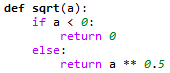
\includegraphics{format_example.png}
  \caption{Pythonコードの強調表示例}
\end{figure}
